%%%%%%%%%%%%%%%%%%%%%%%%%%%%%%%%%%%%%%%%%
% baposter Landscape Poster
% LaTeX Template
% Version 1.0 (11/06/13)
%
% baposter Class Created by:
% Brian Amberg (baposter@brian-amberg.de)
%
% This template has been downloaded from:
% http://www.LaTeXTemplates.com
%
% License:
% CC BY-NC-SA 3.0 (http://creativecommons.org/licenses/by-nc-sa/3.0/)
%
%%%%%%%%%%%%%%%%%%%%%%%%%%%%%%%%%%%%%%%%%

%----------------------------------------------------------------------------------------
%    PACKAGES AND OTHER DOCUMENT CONFIGURATIONS
%----------------------------------------------------------------------------------------

\documentclass[landscape,a0paper,fontscale=0.285]{baposter} % Adjust the font scale/size here

\usepackage{graphicx} % Required for including images
\graphicspath{{figures/}} % Directory in which figures are stored

\usepackage{amsmath} % For typesetting math
\usepackage{amssymb} % Adds new symbols to be used in math mode

\usepackage{booktabs} % Top and bottom rules for tables
\usepackage{enumitem} % Used to reduce itemize/enumerate spacing
\usepackage{palatino} % Use the Palatino font
\usepackage[font=small,labelfont=bf]{caption} % Required for specifying captions to tables and figures

\usepackage{multicol} % Required for multiple columns
\setlength{\columnsep}{1.5em} % Slightly increase the space between columns
\setlength{\columnseprule}{0mm} % No horizontal rule between columns

\usepackage{tikz} % Required for flow chart
\usetikzlibrary{shapes,arrows} % Tikz libraries required for the flow chart in the template

\newcommand{\compresslist}{ % Define a command to reduce spacing within itemize/enumerate environments, this is used right after \begin{itemize} or \begin{enumerate}
\setlength{\itemsep}{1pt}
\setlength{\parskip}{0pt}
\setlength{\parsep}{0pt}
}

\definecolor{lightblue}{rgb}{0.145,0.6666,1} % Defines the color used for content box headers

\begin{document}

\begin{poster}
{
headerborder=closed, % Adds a border around the header of content boxes
colspacing=1em, % Column spacing
bgColorOne=white, % Background color for the gradient on the left side of the poster
bgColorTwo=white, % Background color for the gradient on the right side of the poster
borderColor=lightblue, % Border color
headerColorOne=black, % Background color for the header in the content boxes (left side)
headerColorTwo=lightblue, % Background color for the header in the content boxes (right side)
headerFontColor=white, % Text color for the header text in the content boxes
boxColorOne=white, % Background color of the content boxes
textborder=roundedleft, % Format of the border around content boxes, can be: none, bars, coils, triangles, rectangle, rounded, roundedsmall, roundedright or faded
eyecatcher=true, % Set to false for ignoring the left logo in the title and move the title left
headerheight=0.1\textheight, % Height of the header
headershape=roundedright, % Specify the rounded corner in the content box headers, can be: rectangle, small-rounded, roundedright, roundedleft or rounded
headerfont=\Large\bf\textsc, % Large, bold and sans serif font in the headers of content boxes
%textfont={\setlength{\parindent}{1.5em}}, % Uncomment for paragraph indentation
linewidth=2pt % Width of the border lines around content boxes
}
%----------------------------------------------------------------------------------------
%    TITLE SECTION 
%----------------------------------------------------------------------------------------
%
{
\includegraphics[height=0em]{wits.jpg}} % First university/lab logo on the left
{\bf\textsc{Automated Parking Space Detection}\vspace{0.5em}} % Poster title
{\textsc{ Julien Nyambal (1439552), School of Computer Science \& Applied Mathematics}} % Author names and institution
{
\includegraphics[height=9em]{wits.jpg}} % Second university/lab logo on the right

%----------------------------------------------------------------------------------------
%    OBJECTIVES
%----------------------------------------------------------------------------------------

\headerbox{Abstract}{name=objectives,column=0,row=0}{


Finding a parking space nowadays becomes an issue that is not to neglect, it consumes time and energy. This paper presents an approach for a real-time parking space detection based on Convolutional Neural Networks(CNN) using Caffe and nVidia DiGITS frameworks. Our system checks a defined area whether a parking spot (bounding boxes defined at initialization of the system) is containing a car or not (occupied or vacant).\newline
Our system has been trained using the LeNet network with the Nesterov`s Accelerated Gradient as solver and the AlexNet network with the Stochastic Gradient Descent as solver.

\vspace{0.3em} % When there are two boxes, some whitespace may need to be added if the one on the right has more content
}


%----------------------------------------------------------------------------------------
%    The System
%----------------------------------------------------------------------------------------

%\headerbox{The System}{name=results,column=1,span=2,row=0}{

\headerbox{Data Preparation and Dataset}{name=results,column=1,span=2,row=0}{

\begin{multicols}{2}

\vspace{1em}
\begin{center}
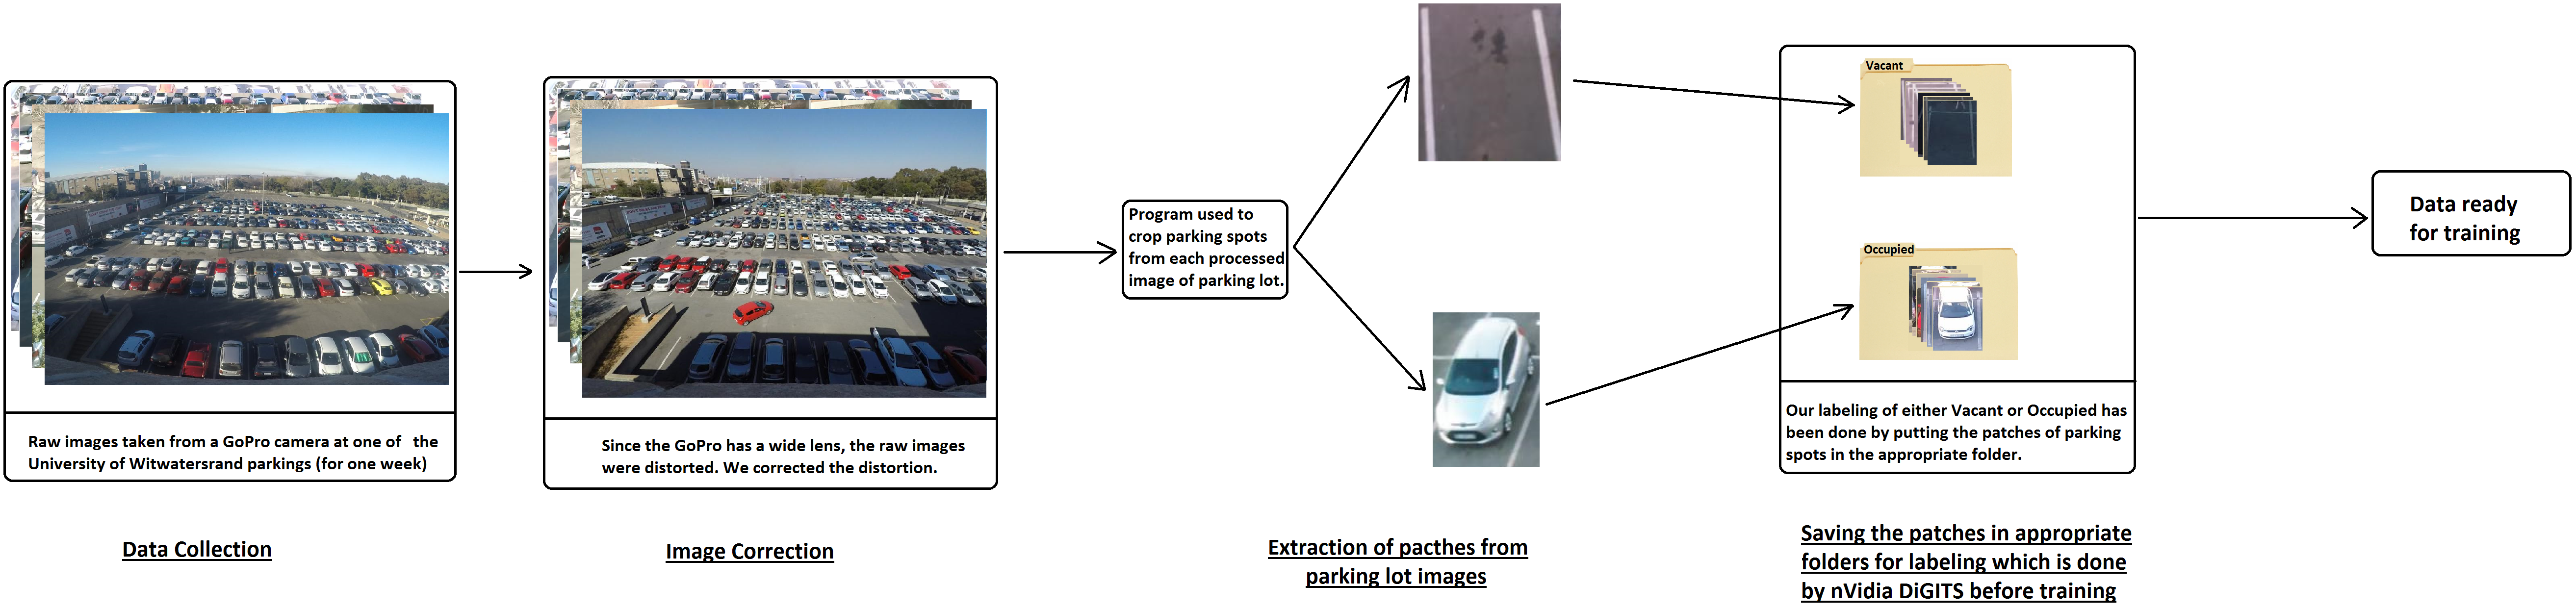
\includegraphics[width=2\linewidth]{dataset}
\captionof*{figure}{}
\end{center}

\end{multicols}

}

%----------------------------------------------------------------------------------------
%    REFERENCES
%----------------------------------------------------------------------------------------

\headerbox{References}{name=references,column=0,above=bottom}{

\renewcommand{\section}[2]{\vskip 0.05em} % Get rid of the default "References" section title
\nocite{*} % Insert publications even if they are not cited in the poster
\small{ % Reduce the font size in this block
%\bibliographystyle{unsrt}
\bibliographystyle{siam}
\bibliography{sample} % Use sample.bib as the bibliography file
}}

%----------------------------------------------------------------------------------------
%    FUTURE RESEARCH
%----------------------------------------------------------------------------------------

\headerbox{Conclusion and Future Work}{name=futureresearch,column=1,span=2,above=bottom}{ % This block is as tall as the references block

\begin{multicols}{2}
Our work has been shown to be very productive and we have produced better results than some other authors. We are planning to improve the parking detection with some perceptive corrections and temporal data to improve accuracy. We will also use artificial intelligence techniques to guide the driver to the closest available parking spot. 

\end{multicols}
}

%----------------------------------------------------------------------------------------
%    CONTACT INFORMATION
%----------------------------------------------------------------------------------------

\headerbox{Contact}{name=contact,column=3,aligned=references,above=bottom}{ % This block is as tall as the references block

\begin{description}\compresslist
\item[Email] Julien.nyambal1@students.wits.ac.za
\item[Phone] +27 83 398 9020
\item [Supervisor] Mr. Richard Klein
\end{description}
}

%----------------------------------------------------------------------------------------
%    Training
%----------------------------------------------------------------------------------------

%\headerbox{Training}{name=conclusion,column=2,span=1,row=0,below=results,above=references}{

\headerbox{Training}{name=conclusion,column=2,span=1,below=results}{

\begin{center}
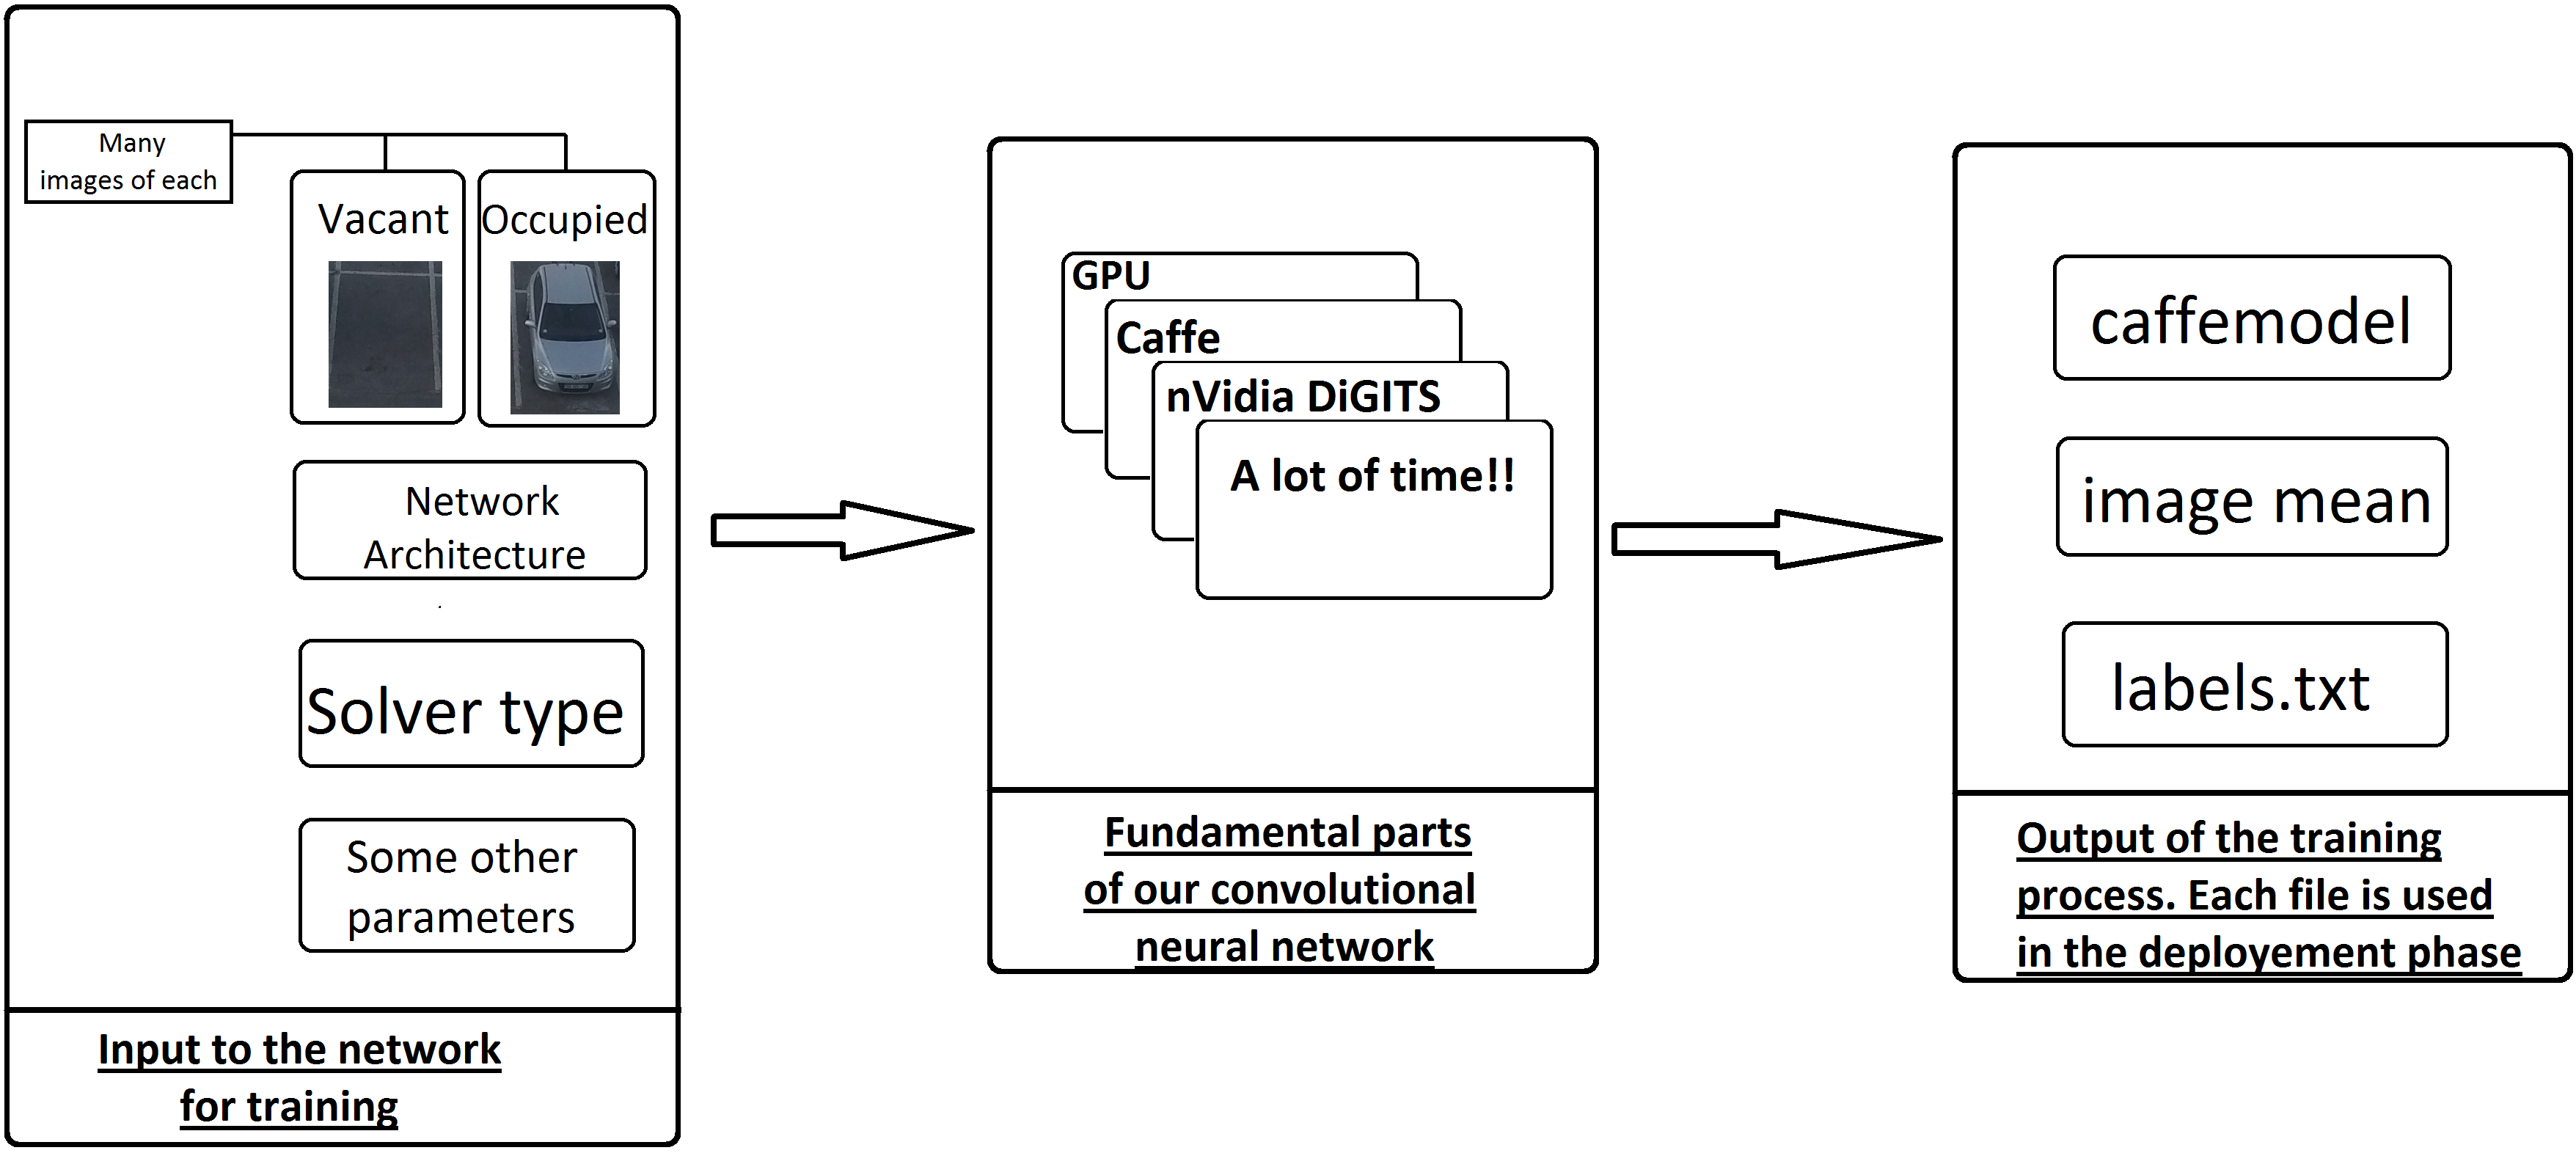
\includegraphics[width=1\linewidth]{training}
\captionof*{figure}{ Training of the classifier}
\end{center}
The classifier is trained from many instances of images of parking spots (vacant and occupied). Some parameters during training include the learning rate, the batch size or customization of the network.

}

%----------------------------------------------------------------------------------------
%    Networks
%----------------------------------------------------------------------------------------

\headerbox{Network Structures}{name=network,column=3,span=1,row=0,above=references}{


\begin{multicols}{2}
\begin{center}
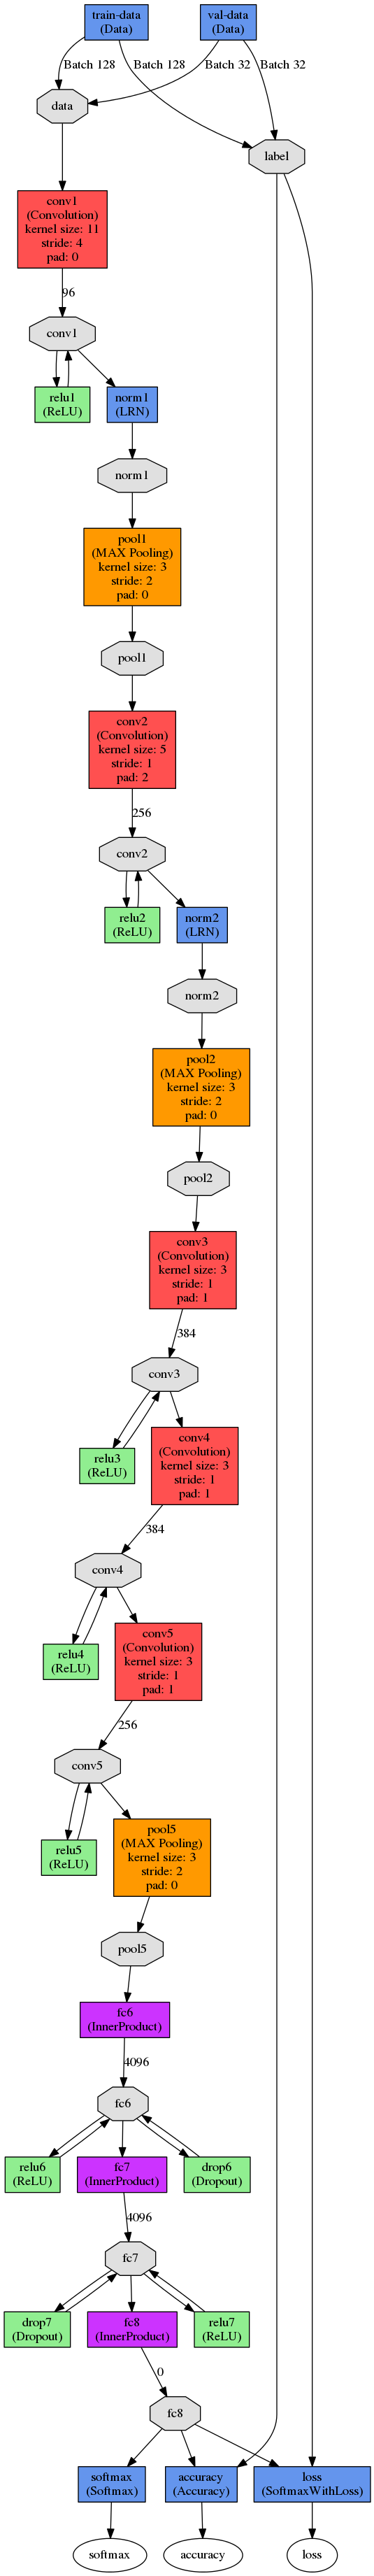
\includegraphics[width=0.65\linewidth]{AlexNet}
\captionof*{figure}{AlexNet}
\end{center}

\begin{center}
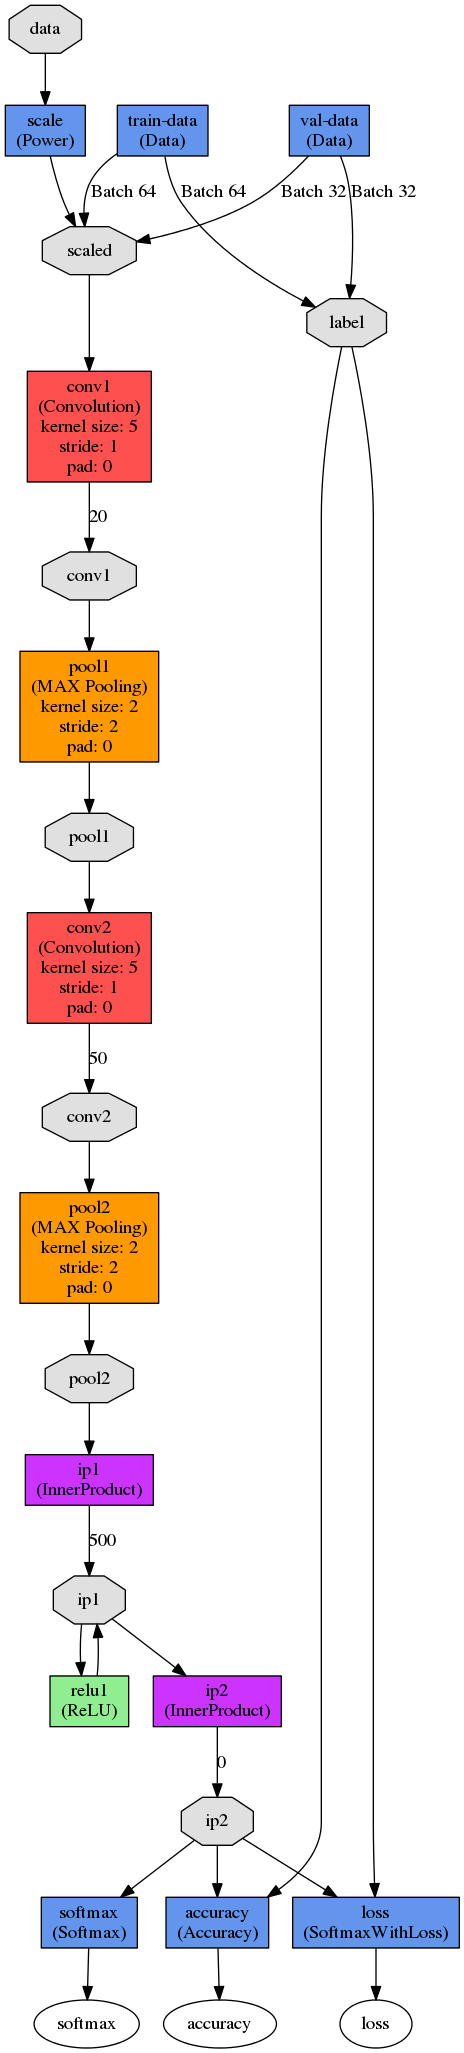
\includegraphics[width=1\linewidth]{LeNet}
\captionof*{figure}{ LeNet}
\end{center}

\end{multicols}
}

%----------------------------------------------------------------------------------------
%    Results
%----------------------------------------------------------------------------------------

%\headerbox{Results}{name=method,column=0,below=objectives,bottomaligned=data}{ % This block's bottom aligns with the bottom of the conclusion block

\headerbox{Results}{name=method,column=0,below=objectives,bottomaligned=network}{ % This block's bottom aligns with the bottom of the conclusion block

We have some good results with most of the architectures used. But for accuracy in detection, we would use the \textbf{AlexNet + SGD}. For speed in processing and high accuracy, we would want to use \textbf{LeNet + NAG}.
The system have been tested on dataset that was totally foreign to the training set. The accuracy remained high, above 90\%.
\begin{center}
\begin{tabular}{l l }
\toprule
\textbf{Network} & \textbf{Accuracy}\\
\midrule
 AlexNet + SGD & 0.95\\ 
 AlexNet + NAG & \textit{Never Ended}\\
 AlexNet + AdaGrad & 0.89\\
 LeNet + SGD & 0.92\\ 
 LeNet + NAG & 0.93\\
 LeNet + AdaGrad & 0.89\\
\bottomrule
\end{tabular}
\captionof{table}{Accuracy calculated from a foreign parking lot}
\end{center}

\begin{center}
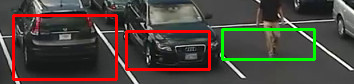
\includegraphics[width=0.8\linewidth]{free1busy}
\captionof*{figure}{System in use}
\end{center}




}

%----------------------------------------------------------------------------------------
%    Algorithm
%----------------------------------------------------------------------------------------

%\headerbox{Algorithm}{name=results2,column=1,span=1,below=results,bottomaligned=conclusion}{ % This block's bottom aligns with the bottom of the conclusion block


\headerbox{Algorithm}{name=results2,column=1,span=1,below=results}{ % This block's bottom aligns with the bottom of the conclusion block

\begin{center}
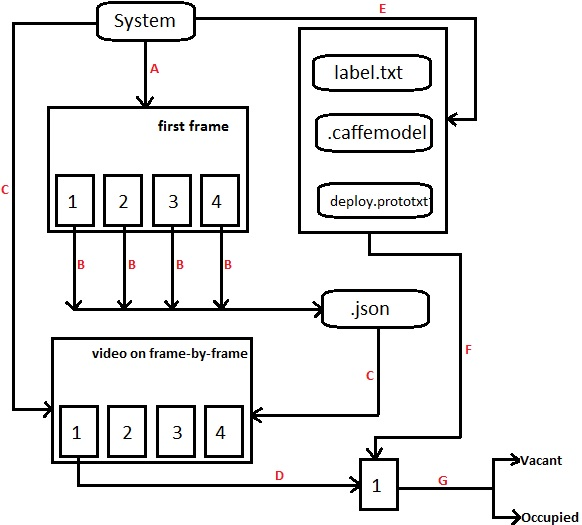
\includegraphics[width=0.5\linewidth]{process}
\captionof*{figure}{Algorithm of the System}
\end{center}

Usage of the trained model, the database of parking spots coordinates on the frames to predict the state of the parking spot. We have to note that the detection is made sequentially. Spot 1, spot2 ...

}



%----------------------------------------------------------------------------------------
%    Dataset
%----------------------------------------------------------------------------------------

%\headerbox{Algorithm}{name=results2,column=1,span=1,below=results,bottomaligned=conclusion}{ % This block's bottom aligns with the bottom of the conclusion block


%\headerbox{Dataset}{name=dataset,column=1,span=2,row=2, below=results2,bottomaligned=network}{ % This block's bottom aligns with the bottom of the conclusion block

\headerbox{System}{name=dataset,column=1,span=2,row=2, below=results2,bottomaligned=network}{ % This block's bottom aligns with the bottom of the conclusion block

\begin{multicols}{2}

\vspace{1em}
\begin{center}
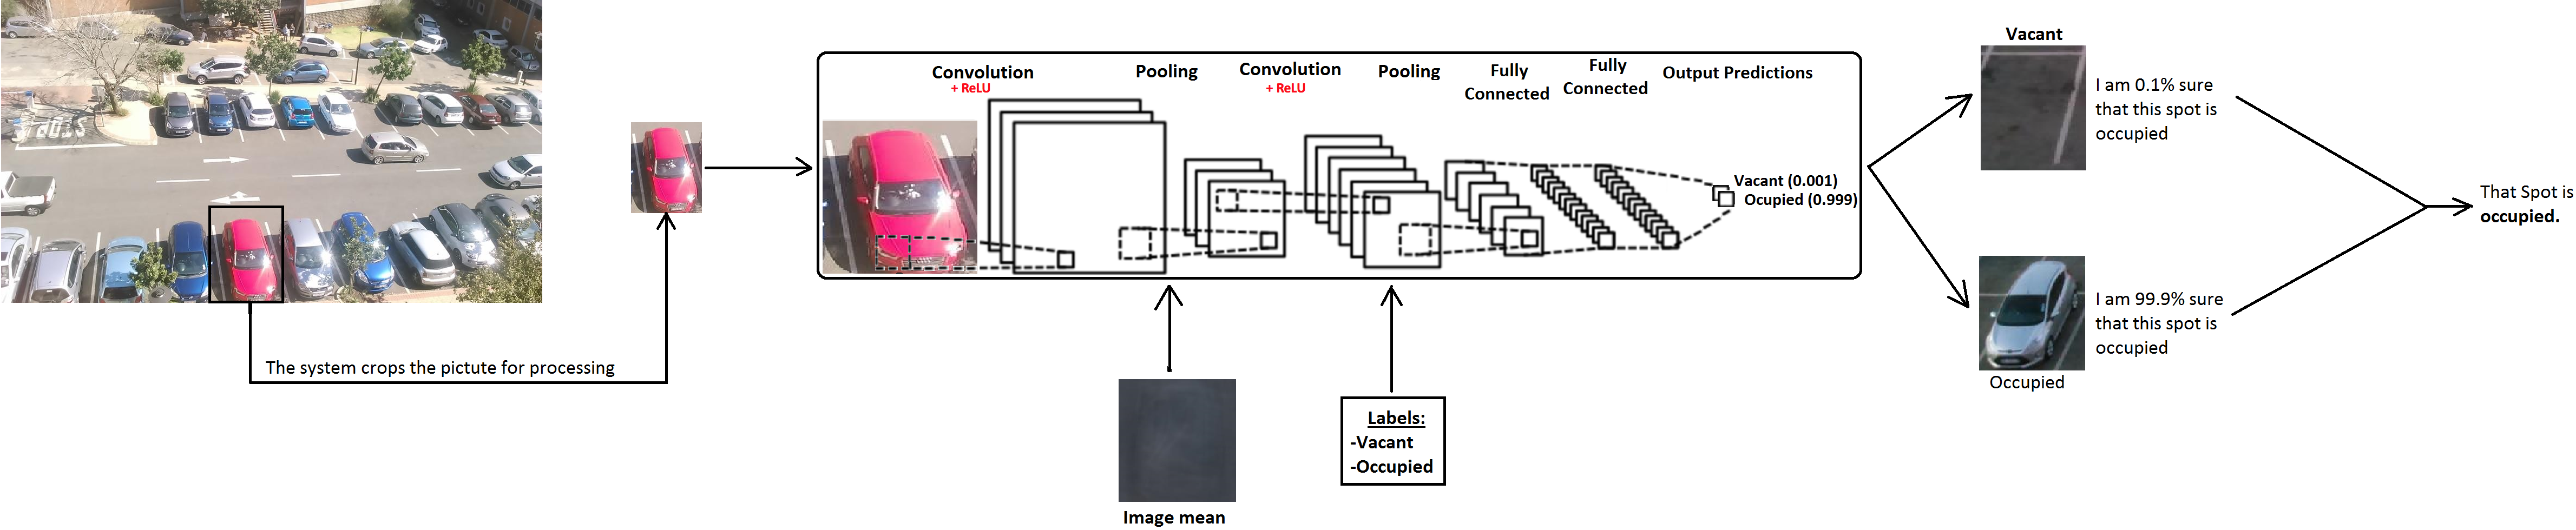
\includegraphics[width=2\linewidth]{system_updated}
\captionof*{figure}{}
\end{center}

\end{multicols}

}




%----------------------------------------------------------------------------------------

\end{poster}

\end{document}